\documentclass[12pt,a4paper]{report}

%====================== PACKAGES ======================

\usepackage[french]{babel}
\usepackage[utf8x]{inputenc}
%pour gérer les positionnement d'images
\usepackage{float}
\usepackage{amsmath}
\usepackage{graphicx}
\usepackage[colorinlistoftodos]{todonotes}
\usepackage{url}
%pour les informations sur un document compilé en PDF et les liens externes / internes
\usepackage{hyperref}
%pour la mise en page des tableaux
\usepackage{array}
\usepackage{tabularx}
%pour utiliser \floatbarrier
%\usepackage{placeins}
%\usepackage{floatrow}
%espacement entre les lignes
\usepackage{setspace}
%modifier la mise en page de l'abstract
\usepackage{abstract}
%police et mise en page (marges) du document
\usepackage[T1]{fontenc}
\usepackage[top=2cm, bottom=2cm, left=2cm, right=2cm]{geometry}
%Pour les galerie d'images
\usepackage{subfig}

%====================== INFORMATION ET REGLES ======================

%rajouter les numérotation pour les \paragraphe et \subparagraphe
\setcounter{secnumdepth}{4}
\setcounter{tocdepth}{4}
\makeatletter
\hypersetup{							% Information sur le document
pdfauthor = {Premier Auteur,
			Deuxième Auteur,
			Troisième Auteur,
    		Quatrième Auteur},			% Auteurs
pdftitle = {Nom du Projet -
			Sujet du Projet},			% Titre du document
pdfsubject = {Mémoire de Projet},		% Sujet
pdfkeywords = {Tag1, Tag2, Tag3, ...},	% Mots-clefs
pdfstartview={FitH}, 					% Ajuste la page à la largueur de l'écran
colorlinks = true, 						% Colorise les liens
breaklinks = true, 						% Permet le retour à la ligne dans les liens trop longs
urlcolor = blue, 						% Couleur des hyperliens
linkcolor = blue, 						% Couleur des liens internes
citecolor = blue,    						% Couleur des liens de citations
bookmarksopen = true,
pdftoolbar = false,
pdfmenubar = false
}					
%pdfcreator = {MikTeX},% Logiciel qui a crée le document
%pdfproducer = {}} % Société avec produit le logiciel

%======================== DEBUT DU DOCUMENT ========================

\begin{document}

%régler l'espacement entre les lignes
\newcommand{\HRule}{\rule{\linewidth}{0.5mm}}

%page de garde

\begin{titlepage}
    \begin{center}
    
    % Upper part of the page. The '~' is needed because only works if a paragraph has started.
    
    \begin{tabular}{cc}
  
\includegraphics[width=0.4\textwidth]{./img/ua_h_couleur}
  \hspace{4cm}
    
\includegraphics[width=0.4\textwidth]{./img/Dpt_Info}
	\end{tabular}    
    
      \vspace{1cm}

	
	
\includegraphics[width=0.4\textwidth]{./img/irset}~\\[1cm]

    
    \textsc{\Large }\\[0.5cm]
    
    % Title
    \HRule \\[0.4cm]
    
    {\huge \bfseries Concrétisation disciplinaire\\
   Projet ESTER \\[0.4cm] }
    
    \HRule \\[1.5cm]
    
    % Author and supervisor
    \begin{minipage}{0.4\textwidth}
    \begin{flushleft} \large
    
     \emph{ESTER:}\\
    Natacha \textsc{Fouquet}\\
    Anna \textsc{Lloyd}\\
    \textsc{\Large }\\[0.3cm]
    \emph{Référents:}\\
    Vincent \textsc{Barichard}\\
    Laurent \textsc{Garcia}
    David \textsc{Genest}
    Jean-Michel \textsc{Richer}
    
    \end{flushleft}
    \end{minipage}
    \begin{minipage}{0.4\textwidth}
    \begin{flushright} \large
    
	\emph{Chefs de projet (M2):}\\
    Hugues \textsc{Dumont}\\
    Guillaume \textsc{Huet}\\
    Zineb \textsc{Loukili}\\
    \textsc{\Large }\\[0.3cm]
    \emph{Équipe de développement (M1):}\\
    Nidal \textsc{Bedyouch}\\
    Imane \textsc{Belhouari}\\
    Théo \textsc{Dézé}\\
    Charles \textsc{Mallet}    
    \end{flushright}
    \end{minipage}
    
    \vfill
    
    % Bottom of the page
    {\large \today}
    
    \end{center}
    \end{titlepage}

%page blanche
\newpage
~
%ne pas numéroter cette page
\thispagestyle{empty}
\newpage

%\input{./abstract.tex}

\tableofcontents
\thispagestyle{empty}
\setcounter{page}{0}
%ne pas numéroter le sommaire

\newpage

%espacement entre les lignes d'un tableau
\renewcommand{\arraystretch}{1.5}

%====================== INCLUSION DES PARTIES ======================

~
\thispagestyle{empty}
%recommencer la numérotation des pages à "1"
\setcounter{page}{0}
\newpage

\chapter{Introduction}

Au cours de ce semestre de Master 1 Informatique, nous avons participé en concrétisation disciplinaire, du développement d'une application ou d'un site web. Nous devions répondre au besoin d'un client, en collaboration avec les Master 2. Ces derniers avaient pour rôle d'organiser les tâches et de gérer toute l'organisation du projet, ainsi que la structure globale. À ce titre, ils étaient les organisateurs et chefs de projet.
En tant que Master 1, nous étions chargés du développement de l'application. Nous devions nous assurer de la bonne implémentation des fonctionnalités et du  bon fonctionnement de l'application.
Dans ce rapport, vous pourrez découvrir l'avancée de notre projet durant ce semestre, selon quatre points. En un premier temps, nous parlerons dans ce compte-rendu de la Gestion de projet suivi Projet côté Serveur. Puis, nous poursuivrons avec la partie côté Client et nous terminerons en abordant les Difficultés et Problèmes rencontrés.




\chapter{Gestion du projet}

\section{Présentation du projet}



\section{Choix technologies}

\subsection{Technologie côté serveur}

\subsubsection{JEE}

Nous avons proposer d'utilisé NodeJS côté serveur, car il s'intègrais particulièrement 
bien a MongoDB et propose une maniere simple d'intégrer des modules. De plus pour la 
parti formation nous aurions du simplement apprendre le javascript et ainsi éviter 
d'apprendre une autre technologie.

Mes nos chefs de projet on décider de choisir le JEE, car c'êtait une technologie 
qu'ils connaissait et cela nous permetais de découvrire la technologie qui nous sera 
utile pour le second semestre.

\subsection{Technologie côté client}


\subsubsection{Highcharts}



\subsection{Base de données}

\subsubsection{Besoin}

Pour le projet, nous avons eu besoin d'une base de données modulaire car un des besoins
était que les questionnaires pouvait évoluer création, modification ou ajout de 
question. Et un autre des besoins était que l'utilisateur puisse faire des sauvegarde 
partiel pour reprendre le questionnaires en case de problème ou si l'utilisateur veut 
faire une pause. 

En plus des besoins spécifique pour la sauvegarde des questionnaires et des réponses. 
Il y a des besoins plus génériques comme la gestion des comptes que nous verrons plus 
en détails dans un autre partie.

\subsubsection{MongoDB}

Nous somme partie sur du MongoDB qui fais partie de la mouvance NoSQL qui s'écarte du 
paradigme classique des bases relationnelles. Cela nous permet de nous affranchir 
d'une des contraintes des base de données SQL qui est de devoir définir un schéma 
prédéfini. Nous somme quand même partie d'un schéma de base pour avoir des données en 
partie structurée.

En offrant un plus grande flexibilité en permettant de gérer des données hétérogènes. 
Dans cas cela est particulièrement utile pour les questionnaires et les réponses car 
si un questionnaires est modifier, il faut que les anciens réponses reste en parti 
utilisable.

\begin{figure}[H]
    \begin{center}
    
\includegraphics[height=2.0cm]{img/mongodb}
    \end{center}
    \caption{Logo de MongoDB}
\end{figure}

Ce choix du type de la base de données a été proposer par nos chefs de projet. La 
raison du choix de MongoDB est car il est le membre le plus populaire de la famille 
NoSQL.   

\section{Planification et répartition des tâches}

\subsection{Outils utilisés}


\subsection{Diagramme de Gantt}


\subsection{Répartitions des rôles}

\chapter{Back-end}
\section{Base de Données}

La base de données est divisée en plusieurs collections.

Pour l'implémentation, nous avons utilisé le driver officiel proposer par MongoDB pour le Java. Nous avons crée une classe mère en Java utilisée par héritage et qui permet de définir des interfaces simplifiant l'utilisation du reste du code.

\subsection{Utilisateur ESTER}

\begin{figure}[H]
    \begin{center}
        \begin{tabularx}{17cm}{|c|X|}
            \hline
            Clé & Valeur  \tabularnewline 
            \hline
            Identifiant & 
            Chaine de caratères, peut être utilisé à la place du mail lors de la connexion \tabularnewline 
            Nom & 
            Chaine de caratères \tabularnewline
            Prénom & 
            Chaine de caratères \tabularnewline
            Première connexion & 
            Boolean \tabularnewline
            Mot de passe & 
            Chaine de caratères chiffrée \tabularnewline
            Mail & 
            Chaine de caratères \tabularnewline
            Statut & 
            Chaine de caratères, représente le statut de l'Utilisateur (Médecin, Administrateur,
            Préventeur, Assistant) \tabularnewline
            \hline
        \end{tabularx}
    \end{center}
    \caption{Tableau de la collection Utilisateur}
\end{figure}

La collection correpond à celle prévue par nos chefs de projet comme
les collections Entreprise et Salarie qui sont des collections proches (L'entreprise ne possède 
pas d'email et le salarie n'a pas de mots de passe mais a la liste des questionnaires répondus ou à répondre
) de Utilisateur ESTER donc nous ne nous répéterons pas. 


\subsection{Questionnaire}

\begin{figure}[H]
    \begin{center}
        \begin{tabularx}{17cm}{|c|X|}
            \hline
            Clé & Valeur  \tabularnewline 
            \hline
            Nom & 
            Nom du questionnaire \tabularnewline 
            Identifiant & 
            Version simplifiée du nom \tabularnewline
            Identifiant ESTER & 
            Identifiant de la personne qui a soumis le questionnaire \tabularnewline
            Date de soumission & 
            Date \tabularnewline
            Mail & 
            Chaine de caratères \tabularnewline
            HTML & 
            Chaine de caratères (HTML brut) \tabularnewline
            \hline
        \end{tabularx}
    \end{center}
    \caption{Tableau de la collection Questionnaire}
\end{figure}

\subsection{Réponse}

\begin{figure}[H]
    \begin{center}
        \begin{tabularx}{17cm}{|c|X|}
            \hline
            Clé & Valeur  \tabularnewline 
            \hline
            Identifiant salarie & 
            Identifiant du salarie qui a répondu \tabularnewline
            Identifiant questionnaire & 
            Identifiant du questionnaire répondu \tabularnewline
            Reponses & 
            Tableau associatif qui lie les identifiants des réponses 
            avec leurs réponses \tabularnewline
            \hline
        \end{tabularx}
    \end{center}
    \caption{Tableau de la colection Réponse}
\end{figure}
\subsection{Sécurité}

Nous stockons des mots de passe dans la base de données, nous avons eu besoin de sécuriser les mots de passe pour ne pas les stocker en clair.
Nous avons comparé plusieurs technologies MD5, SHA256, SHA512, PBKDF2, BCrypt et SCrypt. Ce sont tous des fonctions de hachage mais certaines proposent des bases de salage (PBKDF2, BCrypt, SCrypt) qui permettent de se protéger contre les attaques utilisant des rainbows tables ou par dictionnaire. 
Certaines fonctions de hachage sont difficilement optimisables ce qui permet de rendre plus difficile les attaques par la force brute. De ce fait, cela donne le temps à l'utilisateur de changer sont mot de passe.     

Nous avons choisi d'utilisé BCrypt car il propose une implémentation en java et il fait partie des algorithme les plus sécurisés.
\section{Connexion}

\subsection{Génération chaîne de caractère aléatoire}
    
\begin{itemize} 
\item Problématique :
Lors de la création d’un utilisateur ESTER par un autre (un médecin peut créer un compte infirmier, assistant, préventeur, et un administrateur peut tout créer), un mot de passe provisoire est communiqué à l’utilisateur pour sa première connexion.
D’autre part, le patient se connecte en utilisant un identifiant unique de 5 caractères communiqué par son médecin.
\item  Implémentation :
Pour l’implémentation, nous avons utilisé une instance de la classe SecureRandom \footnote{Cette classe fournit un générateur de nombres aléatoires (RNG) de chiffrement fort.} permettant de tirer aléatoirement les caractères de la chaîne et de la permuter aléatoirement afin d’être imprédictible.
\item  Bilan :
Le générateur de chaîne de caractères aléatoires est fonctionnel et sera utilisé pour la génération de mot de passe provisoire. Tandis que, l’identifiant du patient sera abandonné vu que la complexité de vérification de l’unicité est haute. Les M2 se chargeront de définir un algorithme générant des identifiants cryptés et uniques.

\end{itemize}

\begin{figure}[H]
    \begin{center}
	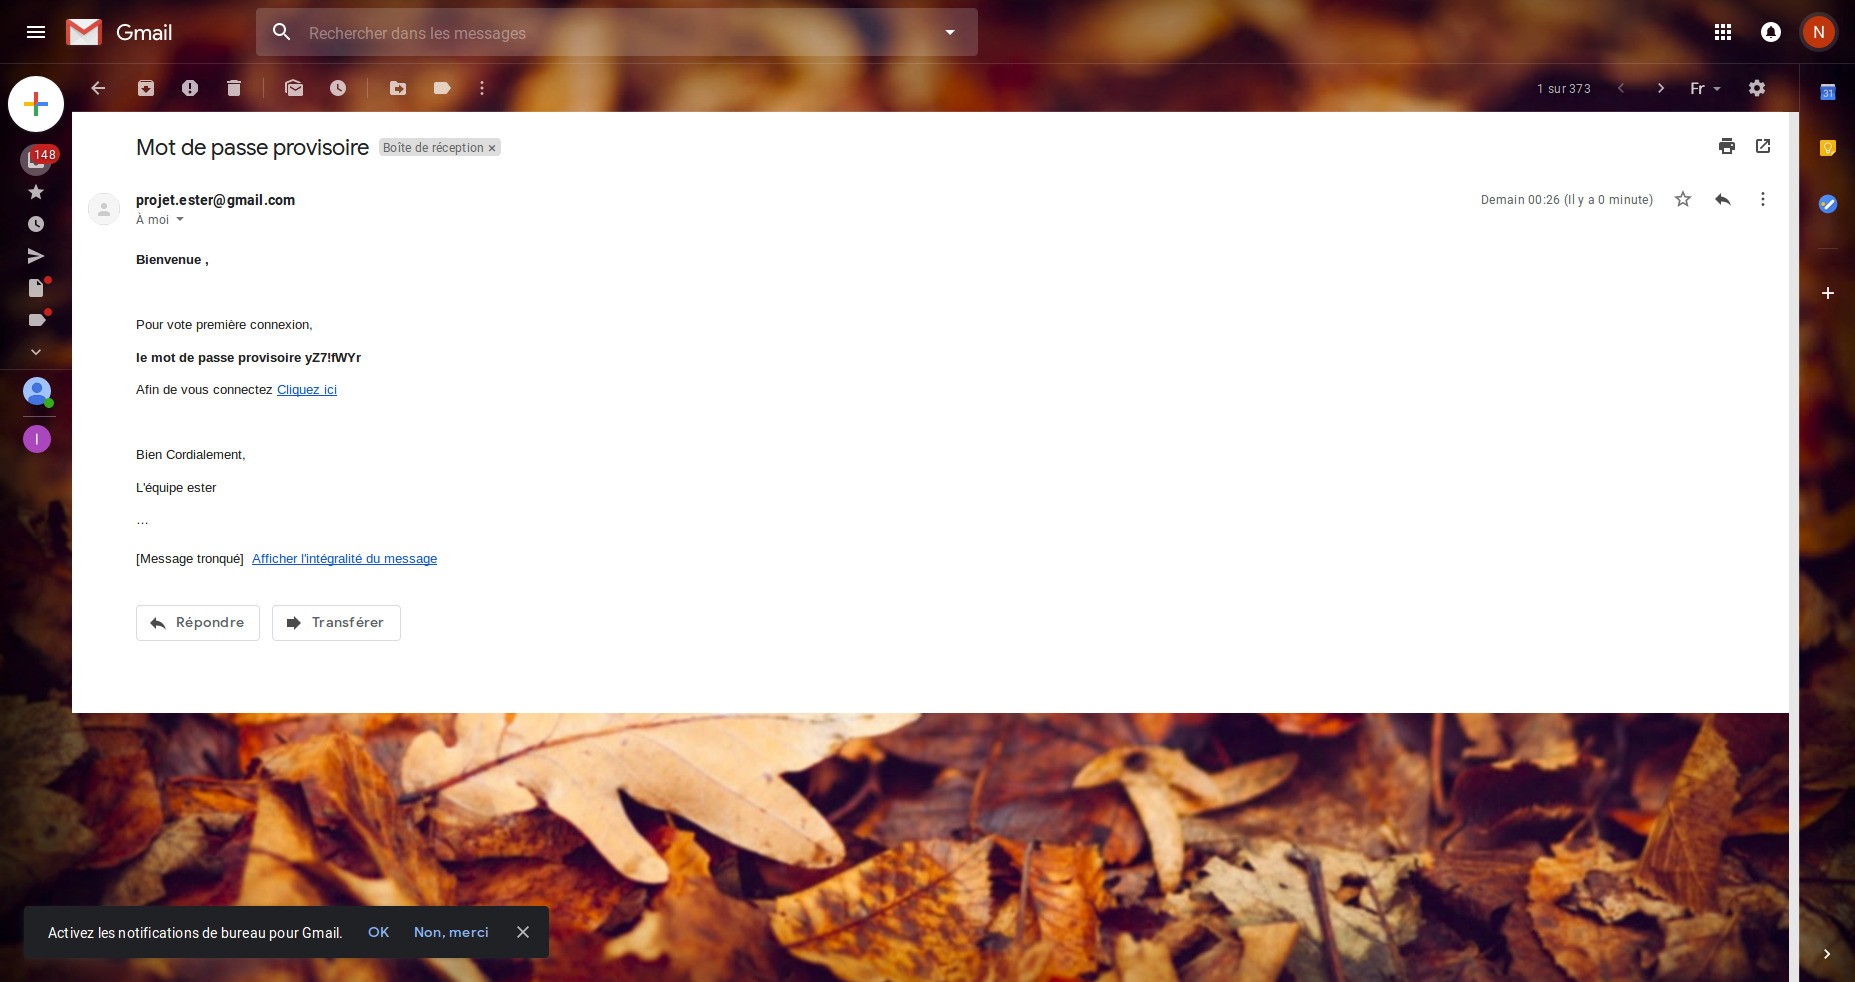
\includegraphics[scale=0.25]{img/connexion/mailCo}
    \end{center}
    \caption{E-mail pour la première connexion}
\end{figure}

\begin{figure}[H]
    \begin{center}
	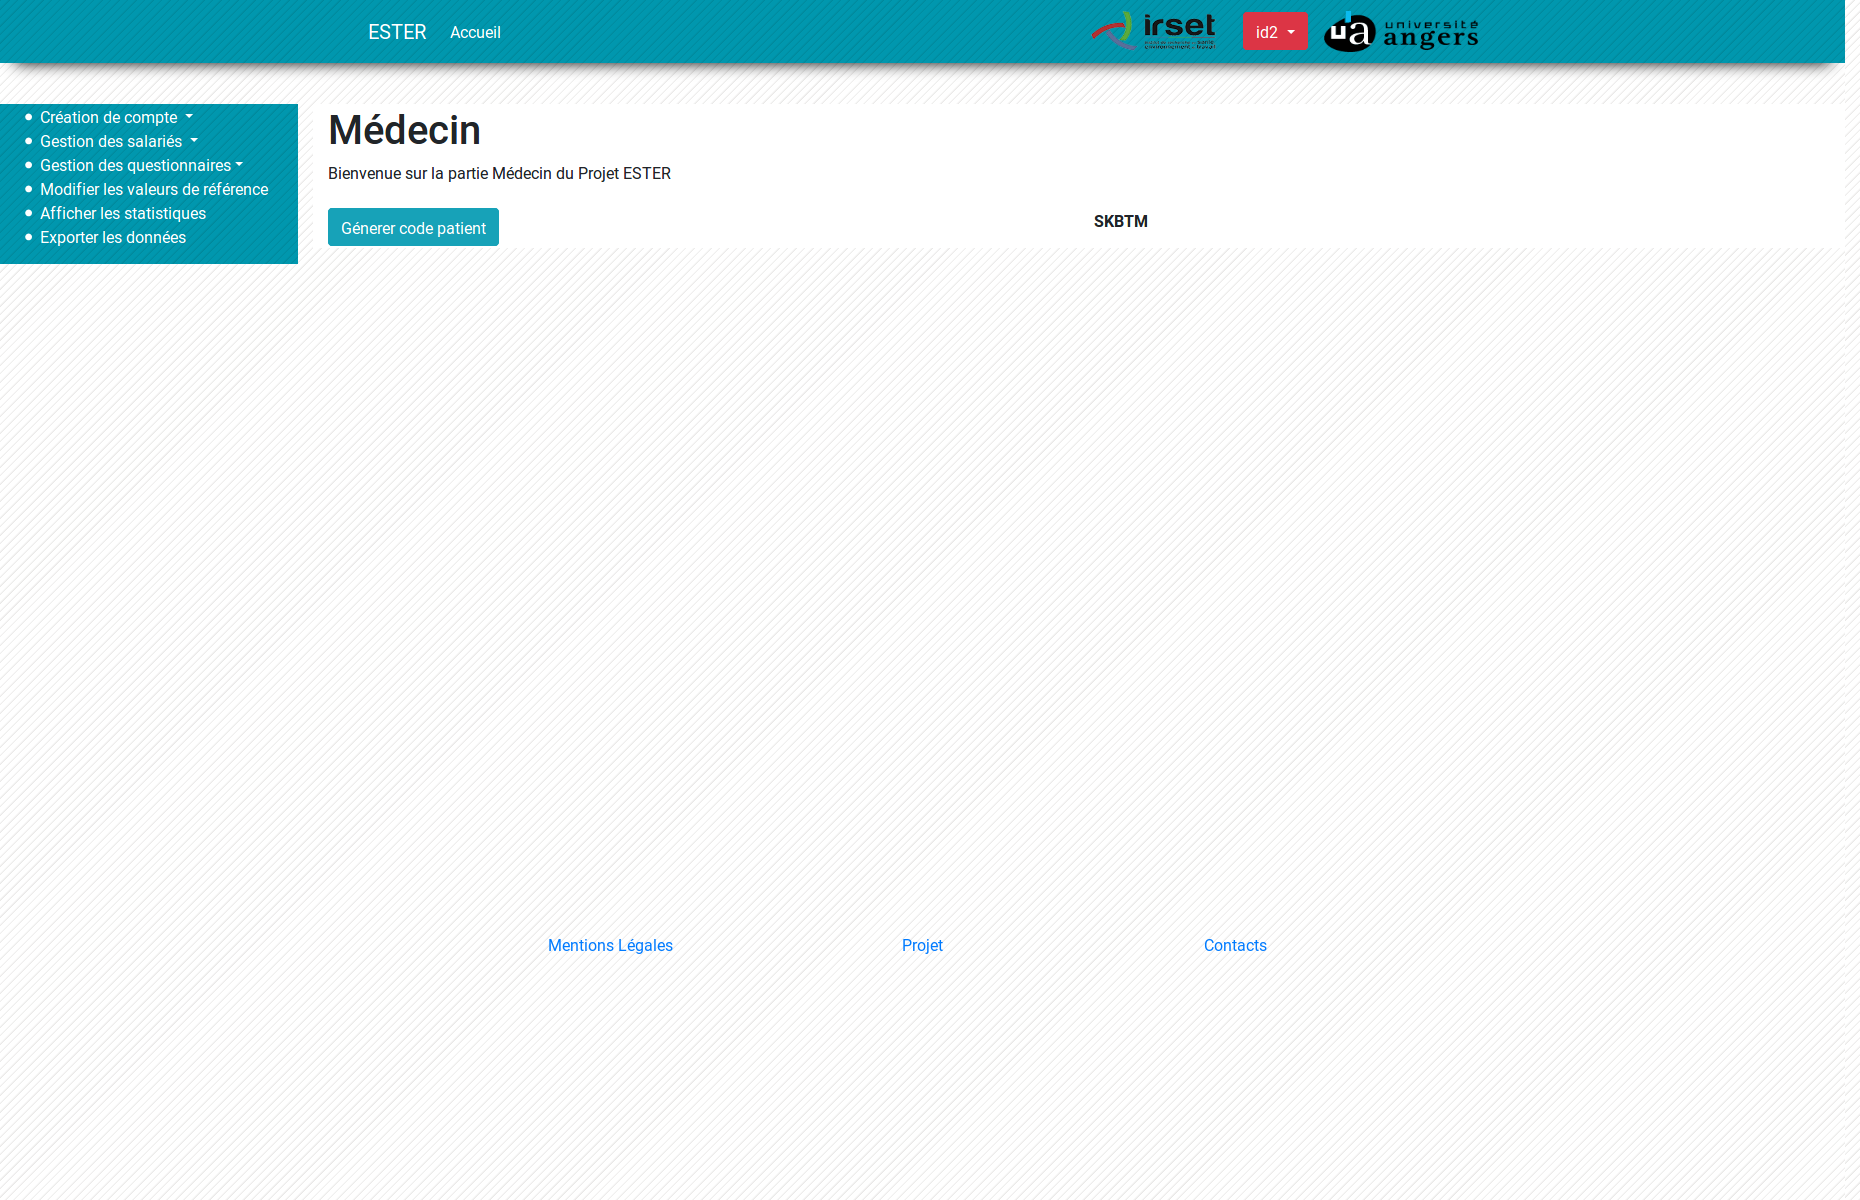
\includegraphics[scale=0.25]{img/connexion/medecin}
    \end{center}
    \caption{Générateur de codes patients}
\end{figure}

\subsection{Formulaire première connexion patient}

Lors de la création d’un compte patient seul l’identifiant est enregistré en base de données. Et afin de compléter les informations manquantes au profil à titre d'illustration: le sexe, l’âge quinquennal (pour préserver l’anonymat du patient), poste de travail, secteur d’activité et département, le patient est redirigé lors de sa première connexion vers le formulaire ci-dessous.

\begin{figure}[H]
    \begin{center}
	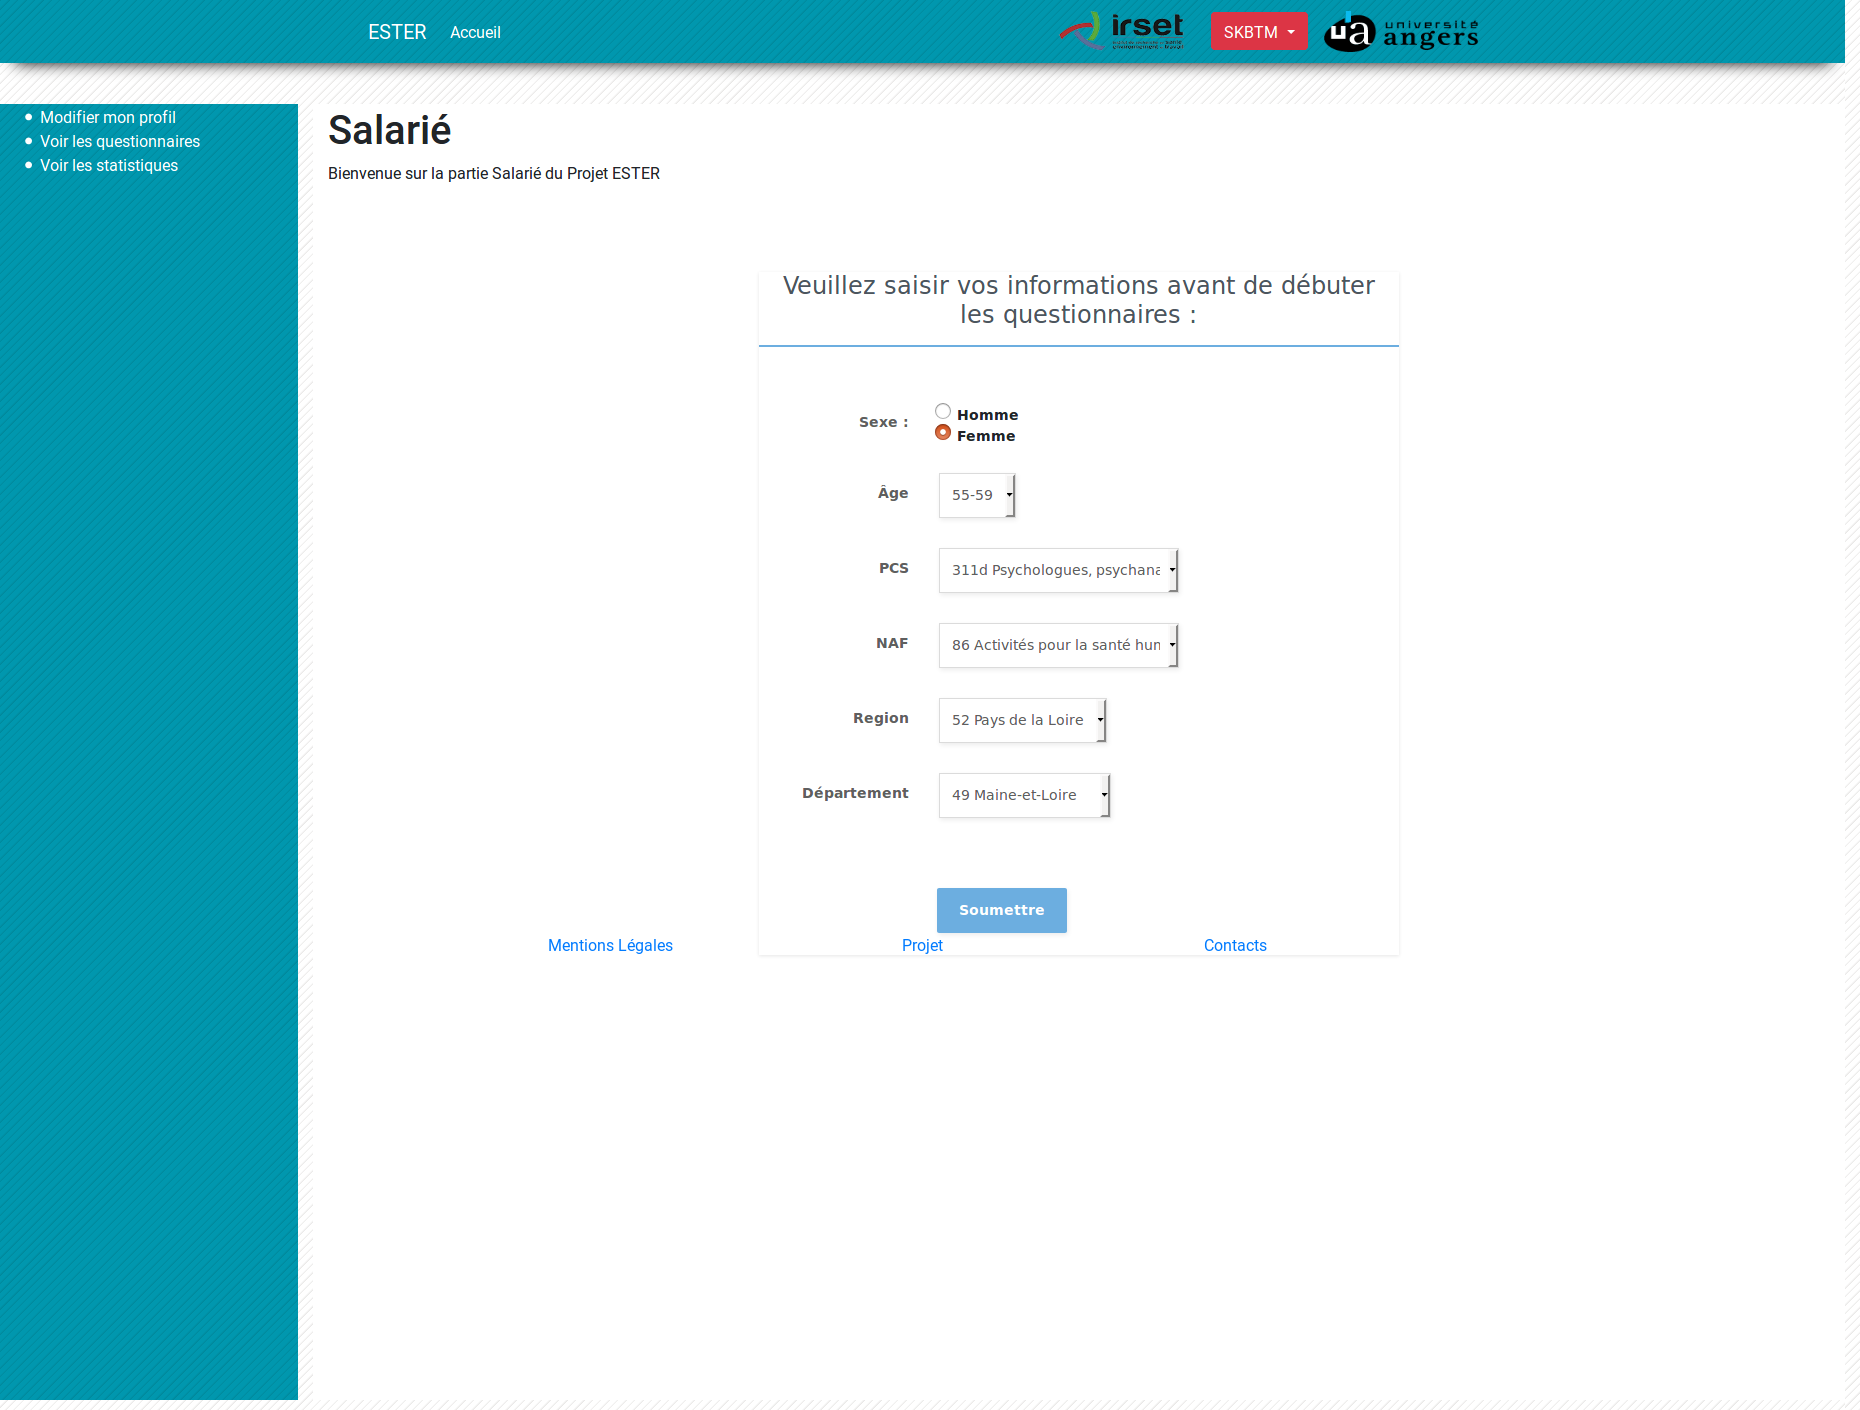
\includegraphics[scale=0.25]{img/connexion/formPatient}
    \end{center}
    \caption{Formulaire du patient à la première connexion}
\end{figure}

\section{Administration e-mail}

\subsection{Envoie Email}

\begin{itemize}

\item Problématique :
Pour la gestion des utilisateurs ester, nous avons eu besoin d’envoyer des emails pour communiquer un mot de passe provisoire pour la première connexion ainsi qu’un lien permettant de réinitialiser le mot de passe.

\item JavaMail API et protocole :
    
\begin{enumerate}


\item JavaMail API :
L'API JavaMail fournit une plateforme indépendante et un Framework de protocoles indépendant pour créer des mails et des applications de messagerie. L'API JavaMail fournit un ensemble de classes abstraites définissant des objets qui constituent un système de messagerie. Il s’agit d’un package optionnel (extension standard) pour la lecture, la composition et l’envoi de messages électroniques. JavaMail fournit des éléments utilisés pour construire une interface avec un système de messagerie, y compris des composants système et des interfaces. Bien que cette spécification ne définisse aucune implémentation spécifique, JavaMail inclut plusieurs classes qui implémentent les normes de messagerie Internet RFC822 et MIME. Ces classes sont livrées dans le cadre du package de classe JavaMail.
\item Protocole SMTP :
SMTP est l'acronyme de Simple Mail Transport Protocol. Ce protocole défini par la recommandation RFC 821 permet l'envoi de mails vers un serveur de mails qui supporte ce protocole.

\end{enumerate}


\item Implémentation :

\begin{enumerate}

\item Envoie email :
L’envoi d’email en utilisant JavaMail API nécessite :
\item Une authentification nécessitant un email, son mot de passe, un hôte et un port.  Pour notre projet en s’est servi du serveur Gmail correspondant à ‘smtp.gmail.com ‘ et le port 587 ;
\item Une instance MimeMessage servant à indiquer destinataire, sujet et corps du message pouvant être en html ou chaîne de caractère.
\item Pour Java9+, il est nécessaire d’ajouter le module activation.jar parce qu’il n’est plus activé par défaut.
\item Configuration serveur mail :
Un compte administrateur peut accéder à l’interface lui permettant de configurer l’envoi d’email en indiquant un email, son mot de passe, un hôte et un port.  
\end{enumerate}


\end{itemize}
    

\subsection{Réinitialisation mot de passe oublié}
	Dans le cadre de la gestion des utilisateurs ester, il s’est avéré important de définir la fonctionnalité réinitialisation de mot de passe. Pour cette fin, nous avons défini deux interfaces, la première sert à indiquer l’email du compte et la deuxième sert définir un nouveau mot de passe.
	Ainsi que l’email de réinitialisation expire dans un délai prédéfini. Pour l’implémenter, nous avons optons pour l’utilisation d’un token unique dans l’URL envoyé en email. Il est généré en utilisant la méthode Java UUID.randomUUID(), qui sert à créer un UUID aléatoire afin d’éviter les collisions. Ainsi ce token est enregistré en base de données en le liant à l’email du compte et la date d’expiration qui à son tour est vérifié lors de l’accès au lien afin de définir sa validité.

\chapter{Front-end}
\section{Structure du site et style}

Chaque page est 

\begin{figure}[H]
    \begin{center}
	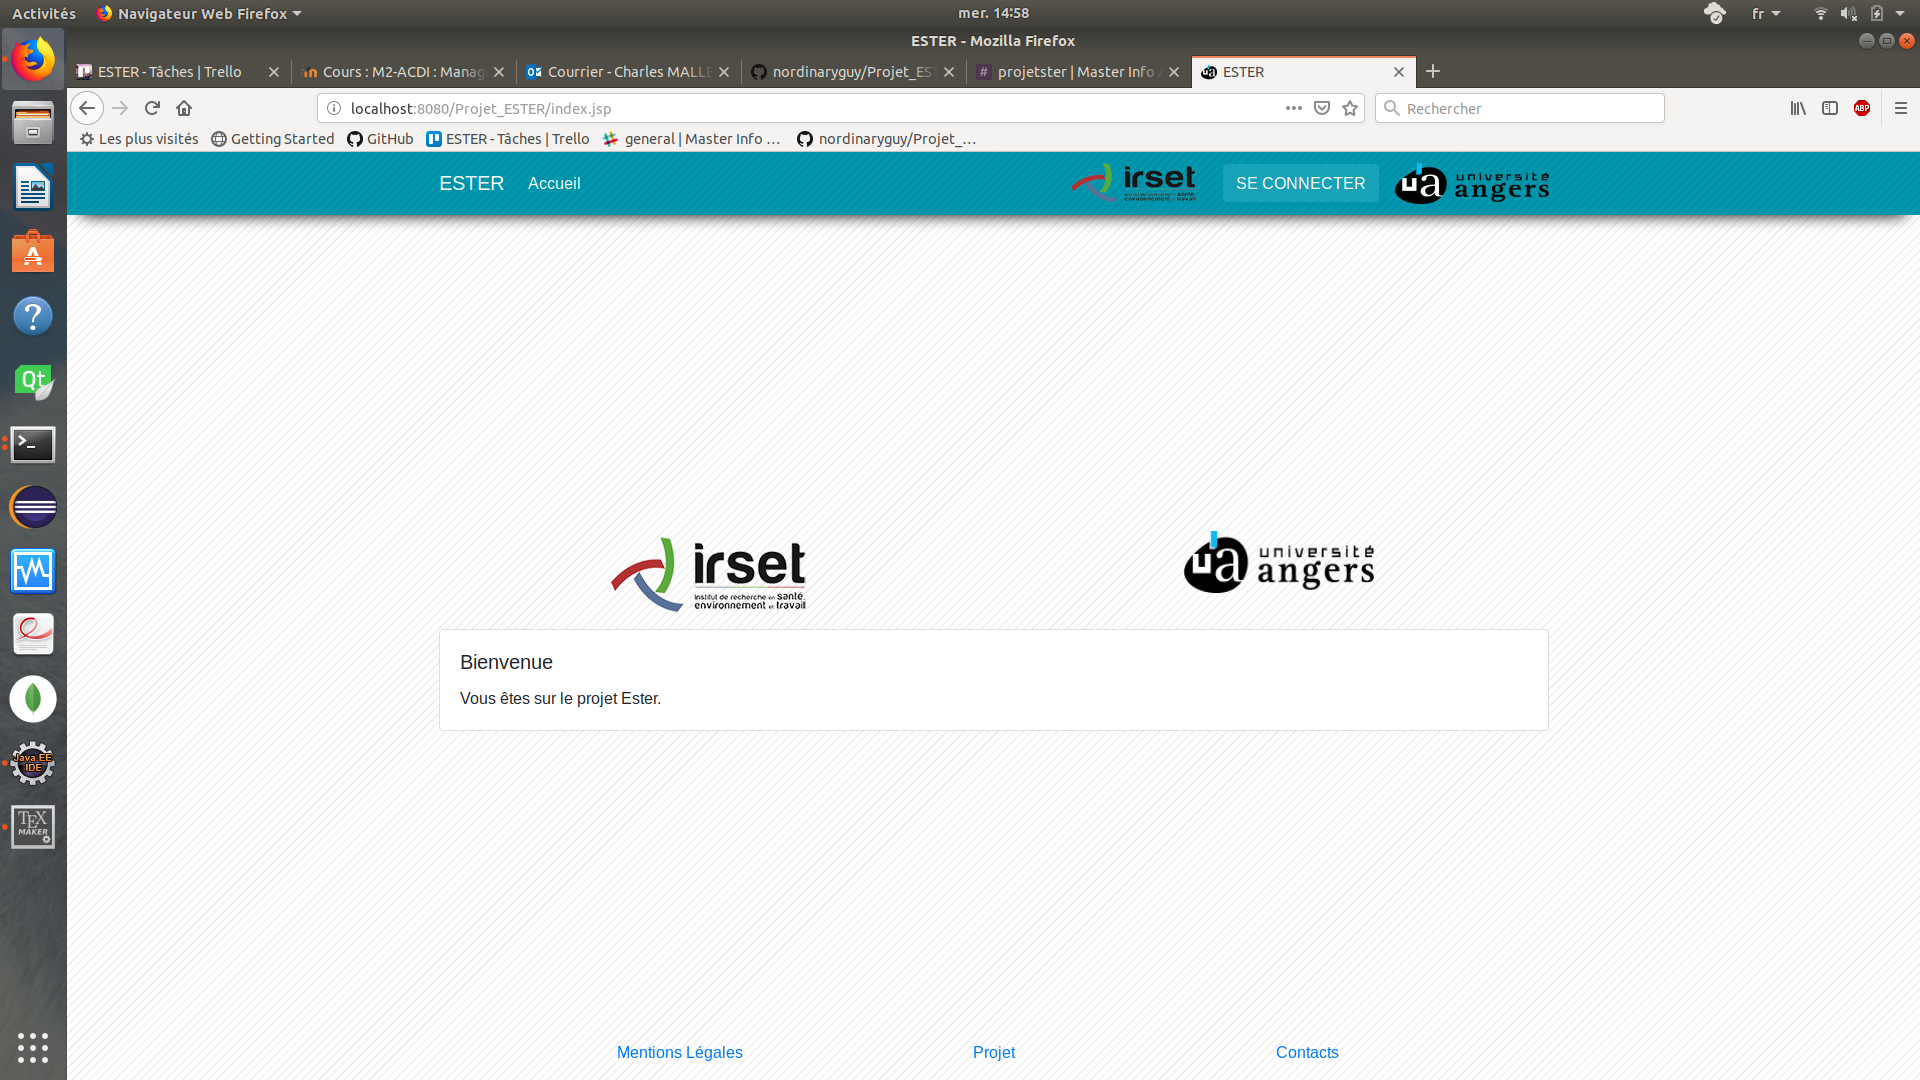
\includegraphics[scale=0.2,trim=4cm 0cm 4cm 5.3cm, clip=true]{img/ESTER}
    \end{center}
    \caption{Page d'Accueil ESTER}
\end{figure}

\begin{figure}[H]
    \begin{center}
	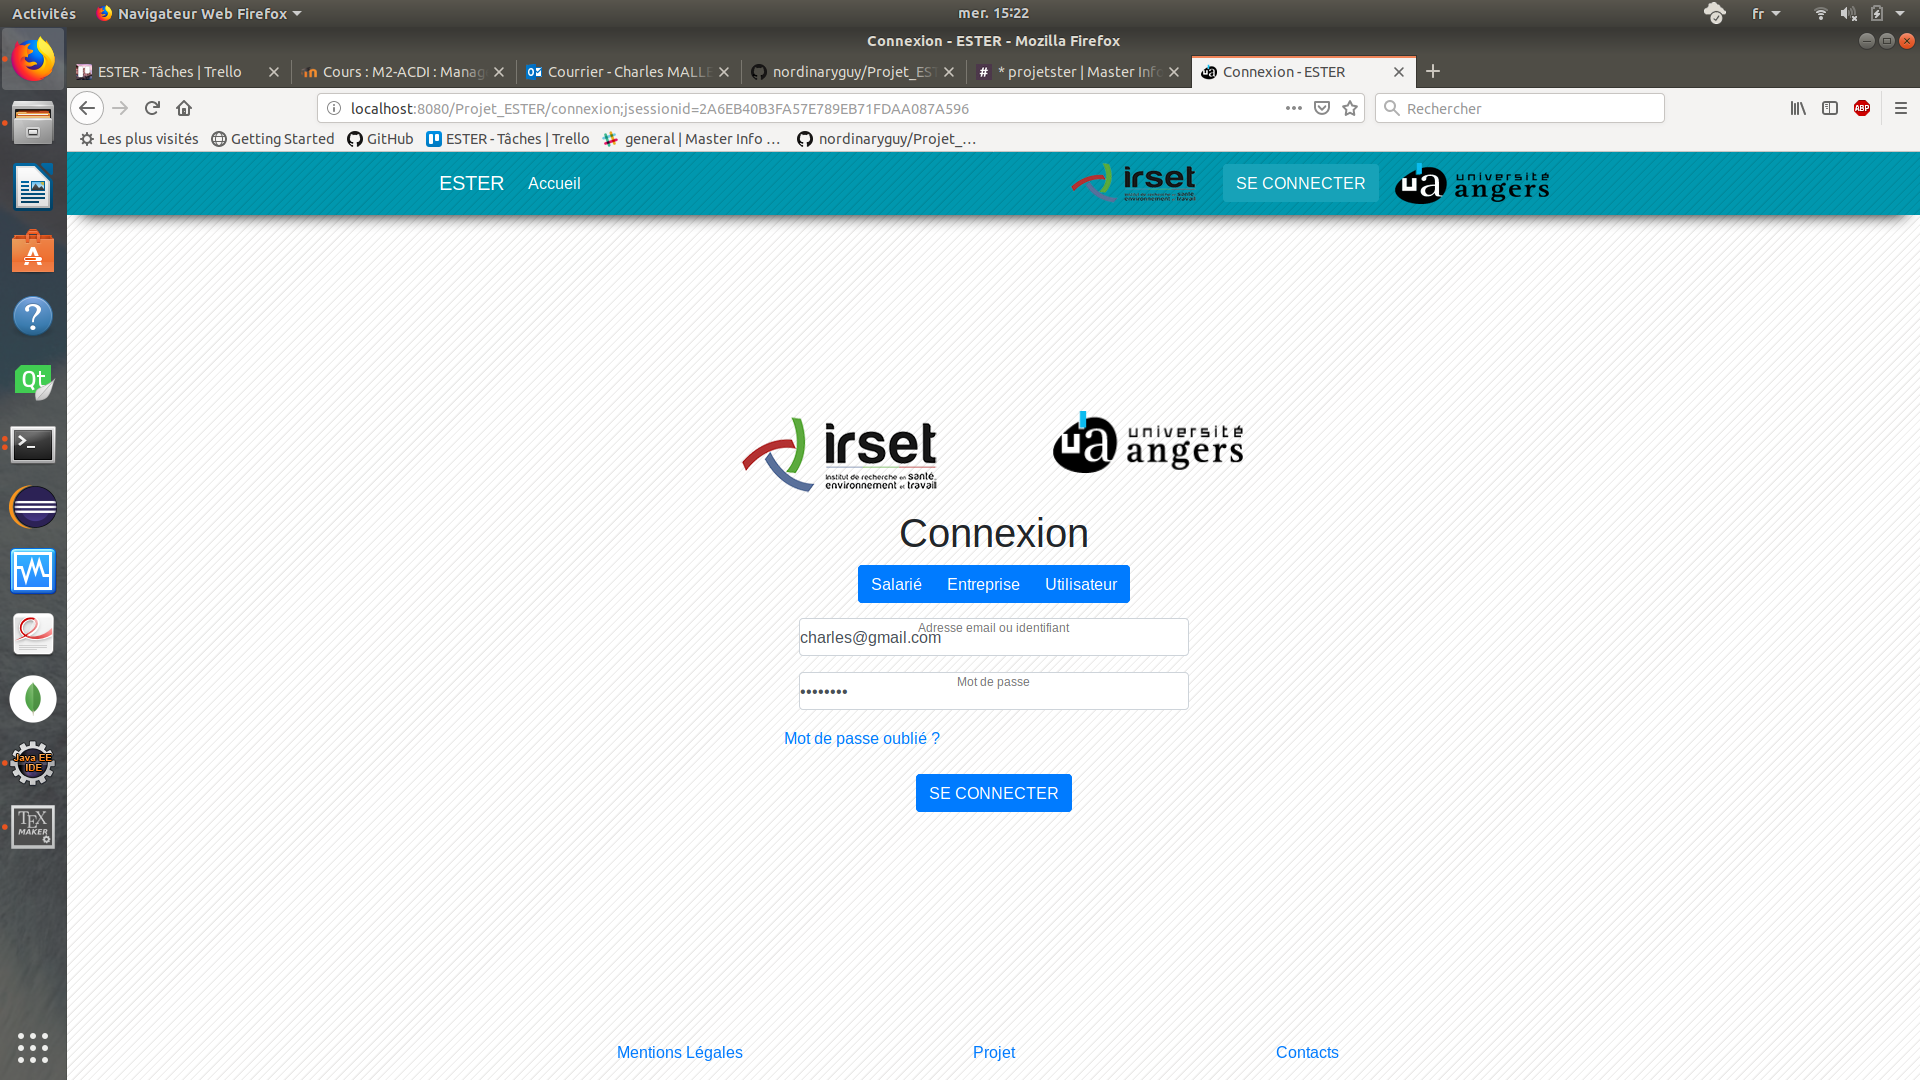
\includegraphics[scale=0.2,trim=4cm 0cm 4cm 5.3cm, clip=true]{img/Connexion}
    \end{center}
    \caption{Page de Connexion}
\end{figure}
\section{Questionnaire}

\subsection{Création de questionnaires}
La problématique consistait à proposer un outil de création de questionnaire facile à
utiliser. Cet outil était un des besoins fondamentaux dans le projet qui nous a été 
donnés. La solution pour répondre au besoin formulé par le client que nous avons adopté, était de créer un générateur de questionnaires. L’utilisateur, à l'aide de celui-ci, peut créer des formulaires HTML en glissé-déposé. Étant donné que les utilisateurs de cet outil sont des non-informaticiens, on a adapté cet outil aux besoins de ces derniers pour le rendre plus facile aussi bien à l’utilisation qu'à la compréhension de son fonctionnement.

\begin{figure}[H]
    \begin{center}
	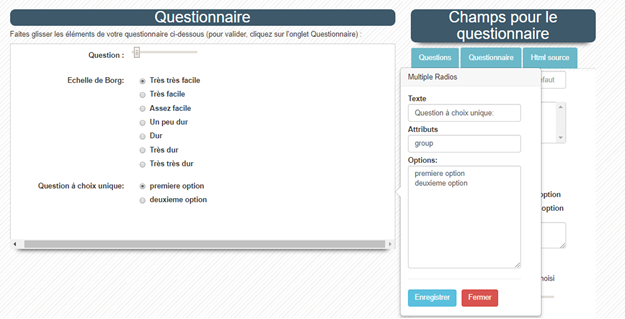
\includegraphics[scale=0.8]{img/questionnaire/modification}
    \end{center}
    \caption{Ajout d'une question dans le générateur de questionnaires}
\end{figure}


\subsection{Outil de création de questionnaire}
\subsubsection{Adaptation du besoin du client}


Cette interface permet à l'utilisateur de créer un questionnaire et paramétrer ses questions en glissant les questions de la partie droite vers la partie gauche et en cliquant sur la question déposée, un nouveau formulaire apparaît avec un nombre de zones de texte différent selon le type de question. Ce formulaire permet de modifier ou remodifier la question.


\begin{figure}[H]
    \begin{center}
	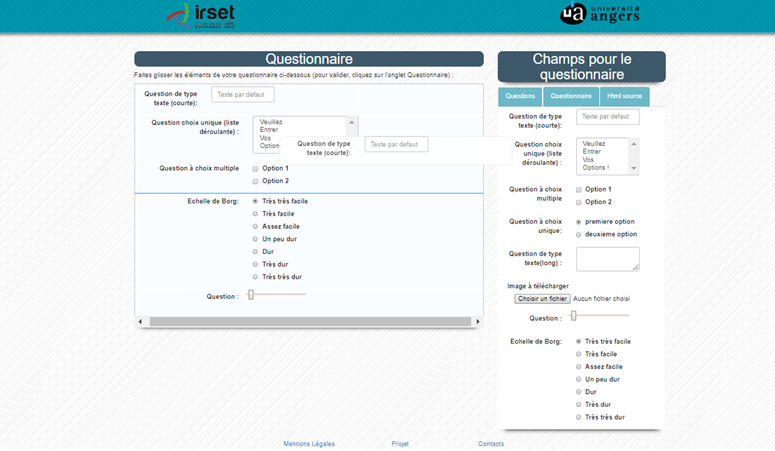
\includegraphics[scale=0.8]{img/questionnaire/generateur}
    \end{center}
    \caption{Modification d'une question}
\end{figure}
 
 
\subsubsection{La gestion des questions}

Pour supprimer une question, il suffit de glisser la question hors du cadre. Cela permet de la retirer des autres questions.


\begin{figure}[H]
    \begin{center}
	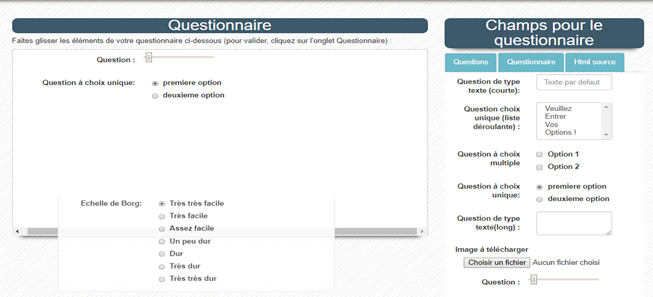
\includegraphics[scale=0.8]{img/questionnaire/suppresion}
    \end{center}
    \caption{Suppression d'une question}
\end{figure}


\subsubsection{Réorganisation des questions}

Lorsqu'on souhaite repositionner les questions, nous avons fait en sorte qu'il suffise de glisser puis déposer les questions à l'endroit où nous souhaitons la placer (en restant dans le même cadre).



\begin{figure}[H]
    \begin{center}
	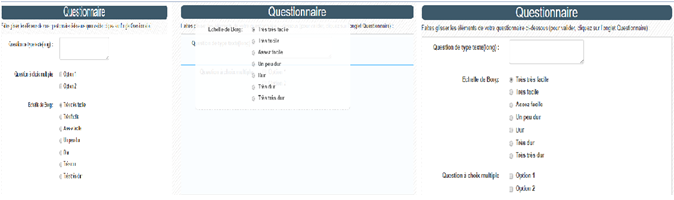
\includegraphics[scale=0.8]{img/questionnaire/repositionnement}
    \end{center}
    \caption{Repositionnement des questions}
\end{figure}

\subsubsection{Sauvegarde du questionnaire}

Pour finaliser la création d’un questionnaire, il faut que l’utilisateur saisisse le nom et l’identifiant du questionnaire puis en cliquant sur le bouton enregistrer. Le questionnaire va être sauvegardé en deux formes différentes, la première est sous forme d’un fichier HTML (figure 3.9) et la deuxième est dans la base de données qu’on peut consulter à partir de la liste des questionnaires (figure 3.10).


\begin{figure}[H]
    \begin{center}
	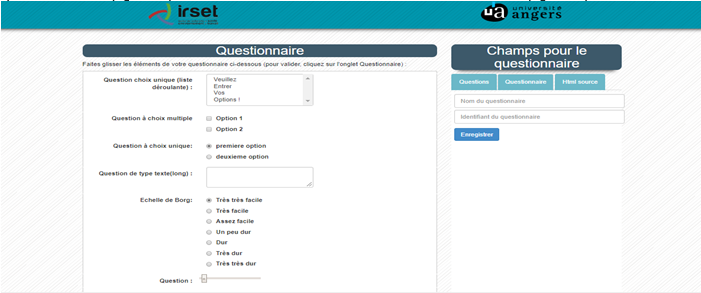
\includegraphics[scale=0.7]{img/questionnaire/enregistrement}
    \end{center}
    \caption{Saisire de données pour finaliser la sauvegarde}
\end{figure}


\begin{figure}[H]
    \begin{center}
	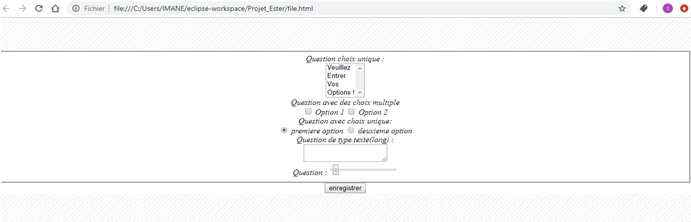
\includegraphics[scale=0.7]{img/questionnaire/fichier}
    \end{center}
    \caption{Sauvegarde sous forme d'un formulaire HTML}
\end{figure}

\begin{figure}[H]
    \begin{center}
	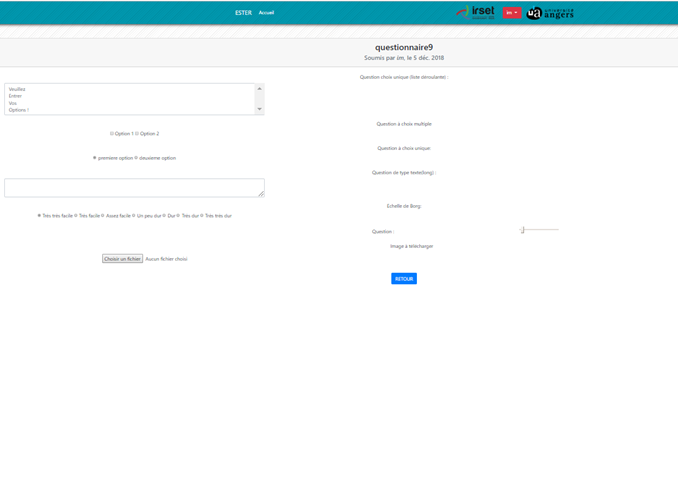
\includegraphics[scale=0.7]{img/questionnaire/affichage}
    \end{center}
    \caption{Affichage du questionnaire enregistré dans la base de données}
\end{figure}
\section{Résultat}

\subsection{Choix}

\subsubsection{Besoin}

Le projet, nous demande une certaine mise en forme (voir figure si dessous) des résultats. Dans les besoins, il avais aussi d'exporter les donnée dans diverses formats CSV, PDF, PNG et autres et d'être compatible avec les PC/Tablette/Smartphone.  

\begin{figure}[H]
    \begin{center}
    
\includegraphics[height=2.0cm]{img/mongodb}
    \end{center}
    \caption{Mise en forme des résultat demandé}
\end{figure}

\subsubsection{Highcharts}

Highcharts est un librairie JavaScript qui permet de généré des graphiques interactifs. Les paramétrages s'effectue en JSON et offre la possibilité export dans les différents formats.

\begin{figure}[H]
    \begin{center}
    
\includegraphics[height=2.0cm]{img/mongodb}
    \end{center}
    \caption{Logo de Highcharts}
\end{figure}

\subsection{Implémentation}

\subsubsection{Highcharts}

L'implémentation de base de Highcharts a été assez simple, mais la création des lignes de séparation (exemple "D'accord vs Pas d'accord") et de coche pour les réponses du le salarie on demandé plus de temps. 

Ce temps en plus est du au temps à la nécessité pour l'adapter a nos besoins. Car certaine n'avais pas des fonctions par défaut pour efféctuer les taches si dessus.

\subsubsection{DWR}

DWR (Direct Web Remoting) est un librairie Java qui permet de recevoir des résultats du serveur sur le principe Ajax (asynchronous JavaScript and XML) qui permet de faire des requêtes aux serveur, mais de manière simplifier.

Cette librairie nous permet de faire le line entre Highcharts et notre serveur pour récupéré les information telle que les questions et leurs valeurs (réponse et pourcentage).

\subsection{Bilan}

Le rendus des résultat est fonctionnel 

\begin{figure}[H]
    \begin{center}
    
\includegraphics[height=2.0cm]{img/mongodb}
    \end{center}
    \caption{Mise en forme des résultat rendus final}
\end{figure}

\chapter*{Conclusion}

Ce projet fut pour nous une véritable nouveauté. Encadré par nos chefs de projets avec qui nous avons eu plusieurs réunions et avec qui nous avons souvent échangés, nous avons pu développer un site web assez important. En dépit des difficultés rencontrés, nous avons essayé de mener notre travail jusqu'à son terme. Le projet ESTER fut pour nous l'occasion de découvrir certaines technologies et de les mettre en application, telles que Bootstrap ou surtout JEE. Le cycle de développement que nous avons suivis, nécessitait une bonne organisation. Que ce soit de définir la base de données, de choisir les technologies ou d'implémenter les fonctionnalités dans le temps imparti, il était impossible de passer outre une certaine rigueur dans le planning. La réalisation de ce site nous a également demandés de faire preuve d'une certaine adaptation et de coordination. 
Nous avons pu constater que travailler dans son coin sur un projet d'une telle importance, n'est pas possible, tout comme prendre les tâches les unes après les autres sans compter sur celles à venir. Nous avons partager nos connaissances, nos visions sur le projet et à ce titre, nous avons pu bien plus appréhender le sujet. Par manque de temps, nous n'avons pas faire aboutir totalement le site. Tout de même, nous sommes parvenus à créer une interface utilisateur correspondant aux attentes de notre client. Nous avons développé un générateur de questionnaires que les médecins pourront prendre en main assez aisément et enregistrer leur travaux. Les salariés peuvent répondre aux questionnaires et les utilisateurs sont en mesure d'accéder aux résultats calculés selon les réponses données par l'utilisateur. Enfin, plusieurs autres fonctionnalités ont été ajoutées à ces principales afin que les utilisateurs puissent mieux s'approprier les pages de notre site.

\newpage

%récupérer les citation avec "/footnotemark"
\nocite{*}

%choix du style de la biblio
\bibliographystyle{plain}
%inclusion de la biblio
\bibliography{bibliographie.bib}
%voir wiki pour plus d'information sur la syntaxe des entrées d'une bibliographie

\end{document}